\chapter{Ficheros del Add-on}
\section{Código Python principal del Add-on}
\label{sec:puntoA1}

\captionsetup{type=listing}
\captionof{listing}{Código python (init.py) principal del panel del add-on.}
\label{lst:panelAddon1}
\begin{minted}[breaklines, fontsize=\small, linenos]{python}
    bl_info = {
        "name": "Chatbot + Generative 3D Assistant",
        "description": "Integra un LLM (streaming/ multihilo) con un Generador 3D en Blender",
        "author": "Víctor Sanz García",
        "version": (0, 7),
        "blender": (3, 6, 0),
        "category": "3D View",
    }
    
    import bpy
    import os
    import threading
    import queue
    import tempfile
    import shutil
    import requests
    import re
    
    from bpy.props import StringProperty
    
    # ----------------------------------------------------------------
    # 1) CÓDIGO DE LLM (streaming + multihilo), FILTRADO DE BARRAS DE CÓDIGO
    # ----------------------------------------------------------------
    
    q = queue.Queue()
    
    # Indicador global para saber si estamos dentro de un bloque de código
    in_code_block = False
    code_python = ""  # Acumula todo el markdown recibido
    code_blocks = []   # Acumula bloques de código extraídos
    
    if __name__ == "blender_GPT":
        from . import streamchatbot
    else:
        import streamchatbot
        from importlib import reload
        reload(streamchatbot)
    
    def extraer_codigo_python():
        """Extrae bloques de código Python del markdown acumulado"""
        global code_python, code_blocks
        
        # Usa el mismo patrón pero con flags para multilínea
        patron = re.compile(r'```[Pp]ython\s*(.*?)```', re.DOTALL)
        bloques = patron.findall(code_python)
        
        # Filtra solo nuevos bloques que no hayamos procesado
        nuevos_bloques = [b.strip() for b in bloques if b.strip() not in code_blocks]
        
        # Actualiza la lista de bloques conocidos
        code_blocks.extend(nuevos_bloques)
        
        return "\n\n".join(nuevos_bloques)
    
    def write_chat(chunk):
        """
        - Toma el fragmento 'chunk' (en Markdown).
        - Filtra para extraer solo las líneas que estén dentro de bloques
          de código (``` ... ```), ignorando todo lo demás.
        - Escribe esas líneas en un Text Editor "ChatBot_Output" y las concatena
          también en scene.response.
        """
        global in_code_block, code_python
    
        text_name = "ChatBot_Output"
    
        # 1) Crear u obtener el Text datablock
        if text_name not in bpy.data.texts:
            text = bpy.data.texts.new(text_name)
            if not bpy.app.background:
                # Abrir el Text Editor
                bpy.ops.screen.userpref_show('INVOKE_DEFAULT')
                for win in bpy.context.window_manager.windows:
                    if win.screen:
                        for area in win.screen.areas:
                            if area.type == 'PREFERENCES':
                                area.ui_type = 'TEXT_EDITOR'
                                area.spaces.active.text = text
        else:
            text = bpy.data.texts[text_name]
    
        # 2) Acumular chunk y extraer código
        global code_python
        code_python += chunk
        
        # Extraer nuevos bloques de código
        nuevo_codigo = extraer_codigo_python()
        
        # 3) Escribir solo si hay nuevo código
        if nuevo_codigo:
            text.write(nuevo_codigo)
            
            # Actualizar solo con el código nuevo
            try:
                scene = bpy.context.scene
                scene.response += nuevo_codigo
            except Exception:
                pass
    
        # 4) Forzar redraw del Text Editor
        for area in bpy.context.screen.areas:
            if area.type == 'TEXT_EDITOR' and area.spaces.active.text == text:
                area.tag_redraw()
    
    
    @bpy.app.handlers.persistent
    def process_queue():
        """
        Timer que se ejecuta cada 0.1 s para vaciar la cola 'q'.
        Cada chunk se manda a write_chat(chunk).
        """
        try:
            while not q.empty():
                chunk = q.get_nowait()
                write_chat(chunk)
        except queue.Empty:
            pass
    
        return 0.1  # Indicamos que queremos volver a ser llamado en 0.1s
    
    
    class ChatBotGenerateOperator(bpy.types.Operator):
        """
        Operador que se dispara al pulsar "Generar código".
        Lanza un hilo que corre create_chat_bot() (que streamea Markdown).
        write_chat() filtrará solo el código Python dentro de ```...```.
        """
        bl_idname = "chatbot.generate_code"
        bl_label = "Generar código"
        bl_description = "Envía el prompt al LLM en un hilo, con streaming"
    
    
        def invoke(self, context, event):
            global in_code_block, code_python, code_blocks
            
            scene = context.scene
            
            # 1) Limpiar respuesta previa y estado
            scene.response = ""
            code_python = ""  # Reiniciar acumulador
            code_blocks = []  # Reiniciar bloques conocidos
    
            # 1) Limpiar respuesta previa y estado de bloques de código
            text_name = "ChatBot_Output"
            if text_name in bpy.data.texts:
                bpy.data.texts.remove(bpy.data.texts[text_name])
            in_code_block = False
    
            # 2) Lanzar el hilo de streaming
            prompt = scene.prompt
            thread = threading.Thread(
                target=streamchatbot.create_chat_bot,
                args=(prompt, "", q)
            )
            thread.daemon = True
            thread.start()
    
            return {'FINISHED'}
    
    
    class ChatBotExecuteOperator(bpy.types.Operator):
        """
        Ejecuta en Blender el código Python que ya está filtrado en scene.response.
        """
        bl_idname = "chatbot.execute_code"
        bl_label = "Ejecutar código"
        bl_description = "Ejecuta en Blender el código generado por el LLM"
    
        def execute(self, context):
            scene = context.scene
            code = scene.response
    
            try:
                exec(code, {'bpy': bpy})
                self.report({'INFO'}, "Código ejecutado correctamente")
            except Exception as e:
                self.report({'ERROR'}, f"Error al ejecutar código: {str(e)}")
    
            return {'FINISHED'}
    
    
    # ----------------------------------------------------------------
    # 2) PROPIEDADES DE SCENE
    # ----------------------------------------------------------------
    
    def init_properties():
        # 2.1) PROPS PARA LLM
        bpy.types.Scene.prompt = StringProperty(
            name="Prompt LLM",
            description="¿Qué acción quieres hacer en Blender?",
            default=""
        )
        bpy.types.Scene.response = StringProperty(
            name="Respuesta LLM",
            description="Aquí aparecerá únicamente el código Python que llegue por streaming",
            default="",
        )
    
        # 2.2) PROPS PARA AGENTE 3D
        bpy.types.Scene.gc_image_path = StringProperty(
            name="Ruta de Imagen",
            description="Ruta de la imagen para generar el modelo 3D",
            default="",
            subtype='FILE_PATH'
        )
        bpy.types.Scene.gc_image_name = StringProperty(
            name="Nombre de Imagen",
            description="Nombre del datablock de la imagen cargada (para preview)",
            default="",
        )
        bpy.types.Scene.gc_model_path = StringProperty(
            name="Ruta de Modelo 3D",
            description="Ruta del archivo 3D generado (.glb)",
            default="",
            subtype='FILE_PATH'
        )
        bpy.types.Scene.gc_status = StringProperty(
            name="Estado Generación",
            description="Estado del proceso de generación 3D",
            default=""
        )
    
    
    def clear_properties():
        # 2.1) LIMPIAR PROPS LLM
        if hasattr(bpy.types.Scene, "prompt"):
            delattr(bpy.types.Scene, "prompt")
        if hasattr(bpy.types.Scene, "response"):
            delattr(bpy.types.Scene, "response")
    
        # 2.2) LIMPIAR PROPS AGENTE 3D
        if hasattr(bpy.types.Scene, "gc_image_path"):
            delattr(bpy.types.Scene, "gc_image_path")
        if hasattr(bpy.types.Scene, "gc_image_name"):
            delattr(bpy.types.Scene, "gc_image_name")
        if hasattr(bpy.types.Scene, "gc_model_path"):
            delattr(bpy.types.Scene, "gc_model_path")
        if hasattr(bpy.types.Scene, "gc_status"):
            delattr(bpy.types.Scene, "gc_status")
    
    
    # ----------------------------------------------------------------
    # 3) OPERADORES DEL AGENTE 3D
    # ----------------------------------------------------------------
    
    class GC_OT_CargarImagen(bpy.types.Operator):
        bl_idname = "gc.cargar_imagen"
        bl_label = "Cargar imagen"
        bl_description = "Selecciona una imagen para generar el modelo 3D"
        filepath: StringProperty(subtype="FILE_PATH")
    
        def execute(self, context):
            scene = context.scene
            path = self.filepath
    
            if os.path.isfile(path):
                try:
                    img = bpy.data.images.load(path)
                    scene.gc_image_path = path
                    scene.gc_image_name = img.name
                    self.report({'INFO'}, "Imagen cargada correctamente")
                except Exception as e:
                    self.report({'ERROR'}, f"Error al cargar imagen: {str(e)}")
            else:
                self.report({'ERROR'}, "La ruta no es válida")
    
            return {'FINISHED'}
    
        def invoke(self, context, event):
            context.window_manager.fileselect_add(self)
            return {'RUNNING_MODAL'}
    
    
    class GC_OT_GenerarModelo3D(bpy.types.Operator):
        bl_idname = "gc.generar_modelo_3d"
        bl_label = "Generar modelo 3D"
        bl_description = "Envía la imagen al servicio 3D y obtiene un archivo GLB de forma no bloqueante"
    
        def invoke(self, context, event):
            scene = context.scene
            image_path = scene.gc_image_path
    
            if not os.path.isfile(image_path):
                self.report({'ERROR'}, "Primero debes cargar una imagen")
                return {'CANCELLED'}
    
            # Limpiar modelo previo
            scene.gc_model_path = ""
    
            # Lanzar hilo para petición HTTP
            thread = threading.Thread(
                target=self.threaded_request_glb,
                args=(image_path,)
            )
            thread.daemon = True
            thread.start()
    
            self.report({'INFO'}, "Petición enviada al servicio 3D (en background)")
            return {'FINISHED'}
    
        def threaded_request_glb(self, image_path):
            try:
                url = "http://127.0.0.1:5000/upload"
                files = {'image': open(image_path, 'rb')}
                response = requests.post(url, files=files, timeout=900)
                response.raise_for_status()
    
                temp_dir = tempfile.gettempdir()
                filename = os.path.join(temp_dir, "gc_model.glb")
                with open(filename, 'wb') as f:
                    f.write(response.content)
    
                # Actualizar en el hilo principal usando propiedades
                def update_success():
                    scene = bpy.context.scene
                    scene.gc_model_path = filename
                    scene.gc_status = f"Modelo 3D generado: {os.path.basename(filename)}"
                    return None
                    
                bpy.app.timers.register(update_success)
    
            except Exception as e:
                # Manejar errores usando propiedades
                def update_error():
                    scene = bpy.context.scene
                    scene.gc_status = f"Error: {str(e)}"
                    return None
                    
                bpy.app.timers.register(update_error)
    
    
    class GC_OT_CargarModelo(bpy.types.Operator):
        bl_idname = "gc.cargar_modelo"
        bl_label = "Cargar modelo"
        bl_description = "Importa el modelo 3D (.glb) generado en la escena"
    
        def execute(self, context):
            scene = context.scene
            model_path = scene.gc_model_path
    
            if not os.path.isfile(model_path):
                self.report({'ERROR'}, "No hay un modelo 3D generado aún")
                return {'CANCELLED'}
    
            try:
                bpy.ops.import_scene.gltf(filepath=model_path)
                self.report({'INFO'}, "Modelo 3D (.glb) importado en la escena")
            except Exception as e:
                self.report({'ERROR'}, f"Error al importar modelo: {str(e)}")
    
            return {'FINISHED'}
    
    
    class GC_OT_DescargarModelo(bpy.types.Operator):
        bl_idname = "gc.descargar_modelo"
        bl_label = "Descargar modelo"
        bl_description = "Guarda una copia del modelo 3D en la ubicación que elijas"
        filepath: StringProperty(subtype="FILE_PATH")
    
        def execute(self, context):
            scene = context.scene
            src = scene.gc_model_path
            dest = self.filepath
    
            if not os.path.isfile(src):
                self.report({'ERROR'}, "No hay un modelo 3D para descargar")
                return {'CANCELLED'}
    
            try:
                shutil.copy(src, dest)
                self.report({'INFO'}, f"Modelo guardado en: {dest}")
            except Exception as e:
                self.report({'ERROR'}, f"Error al guardar modelo: {str(e)}")
    
            return {'FINISHED'}
    
        def invoke(self, context, event):
            if not os.path.isfile(context.scene.gc_model_path):
                self.report({'ERROR'}, "No hay un modelo 3D para descargar")
                return {'CANCELLED'}
            context.window_manager.fileselect_add(self)
            return {'RUNNING_MODAL'}
    
    
    # ----------------------------------------------------------------
    # 4) PANEL PRINCIPAL: AGENTE LLM + AGENTE 3D
    # ----------------------------------------------------------------
    
    class ChatBotPanel(bpy.types.Panel):
        bl_label = "GenerativeCHAT"
        bl_idname = "CHATBOT_PT_panel"
        bl_space_type = 'VIEW_3D'
        bl_region_type = 'UI'
        bl_category = "GenerativeCHAT"
    
        def draw(self, context):
            layout = self.layout
            scene = context.scene
    
            # ==== AGENTE LLM ====
            box_llm = layout.box()
            box_llm.label(text="AGENTE LLM", icon='NODE')
    
            # Input de prompt + botón "Generar código"
            row = box_llm.row(align=True)
            row.prop(scene, "prompt", text="")
            row.operator("chatbot.generate_code", text="Generar código", icon='FILE_SCRIPT')
    
            box_llm.separator()
    
            # Área multiline con la respuesta (solo código Python)
            box_llm.prop(scene, "response", text="")
    
            # Botón "Ejecutar código"
            box_llm.operator("chatbot.execute_code", text="Ejecutar código", icon='PLAY')
    
            # ==== AGENTE 3D ====
            box_3d = layout.box()
            box_3d.label(text="AGENTE 3D", icon='MESH_CUBE')
    
            if scene.gc_status:
                box_3d.label(text=scene.gc_status, icon='INFO')
    
            row3 = box_3d.row()
    
            col_a = row3.column()
            if scene.gc_image_name != "":
                img = bpy.data.images.get(scene.gc_image_name)
                if img:
                    col_a.template_preview(img, show_buttons=False)
            col_a.operator("gc.cargar_imagen", text="Cargar imagen", icon='IMAGE_DATA')
    
            col_b = row3.column()
            col_b.operator("gc.generar_modelo_3d", text="Generar modelo 3D", icon='MOD_REMESH')
    
            if scene.gc_model_path != "":
                box_3d.separator()
                box_3d.label(text=f"Modelo 3D: {os.path.basename(scene.gc_model_path)}", icon='OBJECT_DATA')
                row4 = box_3d.row(align=True)
                row4.operator("gc.cargar_modelo", text="Cargar modelo", icon='IMPORT')
                row4.operator("gc.descargar_modelo", text="Descargar modelo", icon='EXPORT')
    
    
    # ----------------------------------------------------------------
    # 5) REGISTRO / DESREGISTRO
    # ----------------------------------------------------------------
    
    classes = (
        ChatBotGenerateOperator,
        ChatBotExecuteOperator,
        ChatBotPanel,
        GC_OT_CargarImagen,
        GC_OT_GenerarModelo3D,
        GC_OT_CargarModelo,
        GC_OT_DescargarModelo,
    )
    
    def register():
        for cls in classes:
            bpy.utils.register_class(cls)
        init_properties()
    
        # Registro del temporizador para procesar la cola de streaming
        bpy.app.timers.register(process_queue)
    
    
    def unregister():
        # Desregistrar temporizador
        try:
            bpy.app.timers.unregister(process_queue)
        except Exception:
            pass
    
        for cls in reversed(classes):
            bpy.utils.unregister_class(cls)
        clear_properties()
    
    
    if __name__ == "__main__":
        register()
\end{minted}


 
\captionsetup{type=listing}
\captionof{listing}{Código python (streamchatbot.py) generador del stream del chatbot.}
\label{lst:streamBotAddon}
\begin{minted}[breaklines, fontsize=\small, linenos]{python}
    import requests
    import json
    
    def is_json(myjson):
        try:
            json_object = json.loads(myjson)
            return True
        except ValueError as e:
            return False
    
    def create_chat_bot(prompt, key, q): 
        for chunk in chatbot(prompt, key):
            if chunk:
                q.put(chunk)
    
    def chatbot(pmt, key):
        url = "http://127.0.0.1:11434/api/generate"
        
        data = {
            "model": "dolphin-mistral:7b-v2.6-dpo-laser-q4_0",
            "prompt": pmt,
            "stream": True
        }
    
        print("\nTú:", pmt, end="\n\n")
        print("Blender_GPT:", end=" ")
    
        try:
            response = requests.post(url, json=data, stream=True, timeout=900)
            response.raise_for_status()
            
            for line in response.iter_lines():
                if line:
                    try:
                        json_data = json.loads(line)
                        if 'response' in json_data:
                            yield json_data['response']
                    except json.JSONDecodeError:
                        continue
                        
        except Exception as e:
            yield f"\nError: {str(e)}"
\end{minted}



\section{Fichero de inicialización del modelo LLM}
\label{sec:puntoA2}
% Bash
 
\captionsetup{type=listing}
\captionof{listing}{Script Bash (entrypoint.sh) de descarga e inicialización de Ollama y del modelo LLM.}
\label{lst:scriptOllama}
\begin{minted}[breaklines, fontsize=\small, linenos]{bash}
    #!/bin/sh
    
    # Inicia el servidor Ollama en segundo plano
    /bin/ollama serve &
    
    # Espera 20 segundos para que el servidor se inicie
    sleep 20
    
    # Verificar si el modelo está presente
    MODEL_NAME="dolphin-mistral:7b-v2.6-dpo-laser-q4_0"
    if ! ollama list | grep -q "$MODEL_NAME"; then
        echo "Descargando el modelo..."
        
        # Crear un lock file para evitar descargas concurrentes
        LOCK_FILE="/root/.ollama/model_download.lock"
        if [ ! -f "$LOCK_FILE" ]; then
            touch "$LOCK_FILE"
            ollama pull $MODEL_NAME
            rm -f "$LOCK_FILE"
        else
            # Esperar a que otro contenedor complete la descarga
            while [ -f "$LOCK_FILE" ]; do
                echo "Esperando que otro contenedor termine la descarga..."
                sleep 10
            done
        fi
    fi
    
    # Mantener el contenedor en ejecución
    tail -f /dev/null
\end{minted}



\section{Fichero de dependencias del modelo TripoSR}
\label{sec:puntoA3}
  % Quitar cuando esté referenciado
% Imagen requeriments.txt
\captionsetup{type=listing}
\captionof{listing}{Archivo (requirements.txt) de dependencias del modelo 3D.}
\label{lst:dependencias3D}
\begin{minted}[breaklines, fontsize=\small, linenos]{text}
    flask
    flask-cors
    onnxruntime
    gunicorn
    omegaconf==2.3.0
    Pillow==10.1.0
    einops==0.7.0
    transformers==4.35.0
    trimesh==4.0.5
    rembg
    huggingface-hub
    imageio[ffmpeg]
\end{minted}



\section{Ficheros de la API del modelo TripoSR}
\label{sec:puntoA4}
% Código API modelo3d
 
\captionsetup{type=listing}
\captionof{listing}{Código python (app.py) de la API Flask del modelo 3D.}
\label{lst:appAPI3d}
\begin{minted}[breaklines, fontsize=\small, linenos]{python}
    from run import generate_geometry
    from flask import Flask, request, send_file
    from flask_cors import CORS
    import os
    import time
    
    app = Flask(__name__)
    CORS(app)
    
    def check_file_existence(directory, filename):
        """Function to check if a file exists in a directory."""
        return os.path.exists(os.path.join(directory, filename))
    
    @app.route('/upload', methods=['POST'])
    def upload_file():
        if 'image' in request.files:
            image = request.files['image']
            directory = 'output/0'
            filename_mesh = 'mesh.glb'
    
            # Lee los datos binarios de la imagen
            image_data = image.read()
            generate_geometry(image_data)  # Pasa los datos binarios
            
            return send_file(os.path.join(directory, filename_mesh), as_attachment=True, mimetype='model/gltf-binary')
        else:
            return 'No image provided', 400
    
    if __name__ == '__main__':
        app.run(host='0.0.0.0')
\end{minted}



\section{Fichero del modelo TripoSR}
\label{sec:puntoA5}
 
% Código modelo3d adaptado
\captionsetup{type=listing}
\captionof{listing}{Código python (run.py) que ejecuta el modelo 3D adaptado.}
\label{lst:runAPI3d}
\begin{minted}[breaklines, fontsize=\small, linenos]{python}
    import argparse
    import logging
    import os
    import time
    
    import numpy as np
    import rembg
    import torch
    from PIL import Image
    from io import BytesIO
    
    from tsr.system import TSR
    from tsr.utils import remove_background, resize_foreground, save_video
    
    def generate_geometry(image_web):
        class Timer:
            def __init__(self):
                self.items = {}
                self.time_scale = 1000.0  # ms
                self.time_unit = "ms"
    
            def start(self, name: str) -> None:
                if torch.cuda.is_available():
                    torch.cuda.synchronize()
                self.items[name] = time.time()
                logging.info(f"{name} ...")
    
            def end(self, name: str) -> float:
                if name not in self.items:
                    return
                if torch.cuda.is_available():
                    torch.cuda.synchronize()
                start_time = self.items.pop(name)
                delta = time.time() - start_time
                t = delta * self.time_scale
                logging.info(f"{name} finished in {t:.2f}{self.time_unit}.")
    
        timer = Timer()
    
        logging.basicConfig(
            format="%(asctime)s - %(levelname)s - %(message)s", level=logging.INFO
        )
    
        input_image = image_web      #"examples/chair.png"
        output_dir = "output/"
        device = "cuda:0"   #"cpu"
        pretrained = "stabilityai/TripoSR"
        chunksize = 8192
        noremove_bg = False
        foreground = 0.85
        resolution = 256
        model_format = "glb"    #"obj"
        render_store = False
    
        os.makedirs(output_dir, exist_ok=True)
    
        if not torch.cuda.is_available():
            device = "cpu"
    
        timer.start("Initializing model")
        model = TSR.from_pretrained(
            pretrained,
            config_name="config.yaml",
            weight_name="model.ckpt",
        )
        model.renderer.set_chunk_size(chunksize)
        model.to(device)
        timer.end("Initializing model")
    
        timer.start("Processing images")
        images = []
    
        if noremove_bg:
            rembg_session = None
        else:
            rembg_session = rembg.new_session()
    
        if noremove_bg:
            image = np.array(Image.open(BytesIO(input_image)).convert("RGB"))
        else:
            image = remove_background(Image.open(BytesIO(input_image)), rembg_session)
            image = resize_foreground(image, foreground)
            image = np.array(image).astype(np.float32) / 255.0
            image = image[:, :, :3] * image[:, :, 3:4] + (1 - image[:, :, 3:4]) * 0.5
            image = Image.fromarray((image * 255.0).astype(np.uint8))
            if not os.path.exists(os.path.join(output_dir, str(0))):
                os.makedirs(os.path.join(output_dir, str(0)))
            image.save(os.path.join(output_dir, str(0), f"input.png"))
        images.append(image)
        timer.end("Processing images")
    
        for i, image in enumerate(images):
            logging.info(f"Running image {i + 1}/{len(images)} ...")
    
            timer.start("Running model")
            with torch.no_grad():
                scene_codes = model([image], device=device)
            timer.end("Running model")
    
            if render_store:
                timer.start("Rendering")
                render_images = model.render(scene_codes, n_views=30, return_type="pil")
                for ri, render_image in enumerate(render_images[0]):
                    render_image.save(os.path.join(output_dir, str(i), f"render_{ri:03d}.png"))
                save_video(
                    render_images[0], os.path.join(output_dir, str(i), f"render.mp4"), fps=30
                )
                timer.end("Rendering")
    
            timer.start("Exporting mesh")
            meshes = model.extract_mesh(scene_codes, resolution=resolution)
            meshes[0].export(os.path.join(output_dir, str(i), f"mesh.{model_format}"))
            timer.end("Exporting mesh")
\end{minted}



\section{Dockerfile del modelo TripoSR}
\label{sec:puntoA6}
 
% Dockerfile modelo3d
\captionsetup{type=listing}
\captionof{listing}{Dockerfile de la imagen de Docker del servicio del modelo 3D.}
\label{lst:dockerfileM3D}
\begin{minted}[breaklines, fontsize=\small, linenos]{dockerfile}
    # Utiliza una imagen base de Python
    FROM python:3.8-slim
    
    # Establece el directorio de trabajo en el contenedor
    WORKDIR /app
    
    # Copia los archivos de la aplicación Flask al contenedor
    COPY . /app
    
    # Actualiza setuptools y luego instala las dependencias de Python
    RUN pip install --upgrade setuptools && pip install -r requirements.txt && pip install torch torchvision torchaudio -f https://download.pytorch.org/whl/torch_stable.html
    
    # Cambia al directorio del repositorio
    WORKDIR /app/torchmcubes
    
    RUN apt-get update && \
        apt-get install -y g++ ninja-build && \
        apt-get clean && \
        rm -rf /var/lib/apt/lists/*
    
    # Ejecuta el script de Python que genera la carpeta y el archivo .pyd
    RUN python setup.py build_ext -i
    
    # Mueve los archivos generados a la carpeta de librerías de Python
    RUN mv torchmcubes /usr/local/lib/python3.8/site-packages/torchmcubes && \
        mv build/lib.linux-x86_64-cpython-38/
        torchmcubes_module.cpython-38-x86_64-linux-gnu.so 
        /usr/local/lib/python3.8/site-packages/
    
    WORKDIR /app
    
    RUN rm -rf torchmcubes
    
    # Expone el puerto en el que se ejecutará la aplicación Flask
    EXPOSE 5000
    
    # Ejecuta la aplicación Flask con Gunicorn para producción
    CMD ["gunicorn", "-b", "0.0.0.0:5000", "--timeout", "1000", "app:app"]
\end{minted}



\chapter{Ficheros de despliegue local}
\section{Archivos de configuración}
\label{sec:puntoB1}
 
% docker-compose.yml
\captionsetup{type=listing}
\captionof{listing}{Archivo de configuración Docker-Compose del despliegue del servidor en local.}
\label{lst:composeServidor}
\begin{minted}[breaklines, fontsize=\small, linenos]{yaml}
    version: '3.8'
    
    services:
      ollama:
        image: ollama/ollama
        volumes:
          - ollama_data:/root/.ollama
          - ./ollama/entrypoint.sh:/entrypoint.sh
        entrypoint: /entrypoint.sh
        networks:
          - backend
        deploy:
          resources:
            limits:
              memory: 4G  # Más espacio para cargar modelos grandes
            reservations:
              memory: 1G
    
      modelo3d:
        build:
          context: ./modelo3d
        networks:
          - backend
        deploy:
          replicas: 2
          resources:
            limits:
              memory: 6G  # Más memoria para cada instancia
            reservations:
              memory: 3G
    
      nginx:
        image: nginx:alpine
        ports:
          - "11434:80"
          - "5000:5000"
        volumes:
          - ./nginx/nginx.conf:/etc/nginx/nginx.conf
        depends_on:
          - ollama
          - modelo3d
        networks:
          - backend
        environment:
          - NGINX_WORKER_PROCESSES=4
        deploy:
          resources:
            reservations:
              memory: 256M
    
    volumes:
      ollama_data:
    
    networks:
      backend:
        driver: bridge
\end{minted}

 
% nginx.conf
\captionsetup{type=listing}
\captionof{listing}{Archivo de configuración Nginx (nginx.conf) del proxy del servidor.}
\label{lst:nginxConfig}
\begin{minted}[breaklines, fontsize=\small, linenos]{nginx}
    events {
        worker_connections 1024;
    }
    
    http {
        # DNS de Docker para balanceo automático
        resolver 127.0.0.11 valid=10s;
    
        upstream ollama_servers {
            server ollama:11434;
        }
    
        upstream modelo3d_servers {
            server modelo3d:5000;
        }
    
        server {
            listen 80;
            
            location /api/generate {
                proxy_pass http://ollama_servers;
                proxy_http_version 1.1;
                proxy_set_header Host $host;
                proxy_set_header Connection '';
                
                # Timeouts extendidos
                proxy_connect_timeout       900;
                proxy_send_timeout          900;
                proxy_read_timeout          900;
                send_timeout                900;
            }
        }
    
        server {
            listen 5000;
            
            location /upload {
                proxy_pass http://modelo3d_servers;
                proxy_http_version 1.1;
                proxy_set_header Host $host;
                proxy_set_header Connection '';
                client_max_body_size        100M;
                
                # Timeouts extendidos para generación 3D
                proxy_connect_timeout       900;
                proxy_send_timeout          900;
                proxy_read_timeout          900;
                send_timeout                900;
            }
        }
    }
\end{minted}



\chapter{Resultados de pruebas}
\section{Resultados de las pruebas funcionales}
\label{sec:puntoC1}
% Imagen
  \begin{figure}[h!tb]
    \centering
    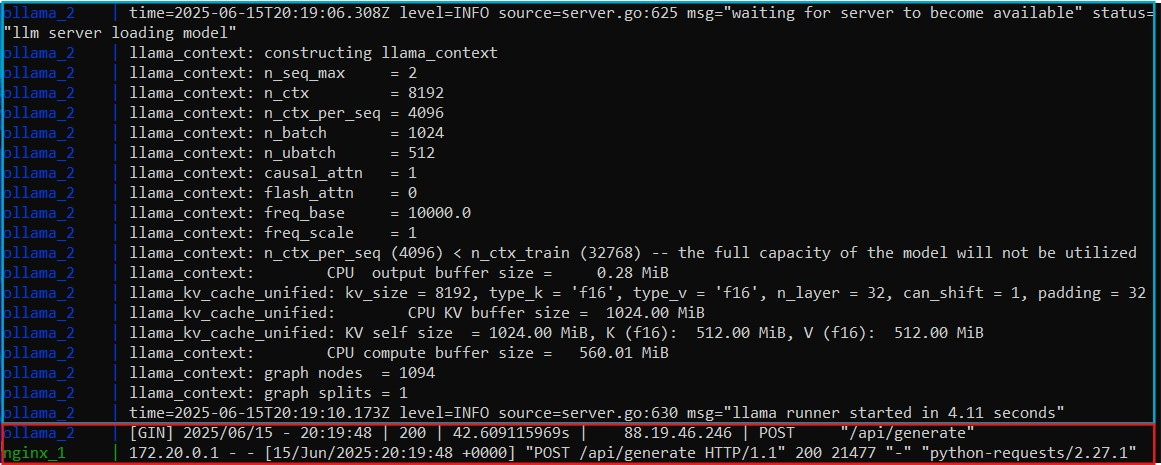
\includegraphics[width=0.8\textwidth]{figs/cu1cu8.jpg}
    \caption{Captura de pantalla del terminal de logs del servidor para el CU1 y CU8 en las pruebas funcionales}
    \label{fig:cu1cu8}
  \end{figure}

% Imagen
  \begin{figure}[h!tb]
    \centering
    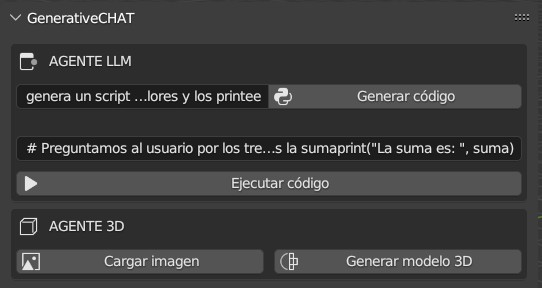
\includegraphics[width=0.8\textwidth]{figs/cu2_1.jpg}
    \caption{Captura de pantalla del campo de respuesta del modelo LLM en el add-on para el CU2 en las pruebas funcionales}
    \label{fig:cu2_1}
  \end{figure}

% Imagen
  \begin{figure}[h!tb]
    \centering
    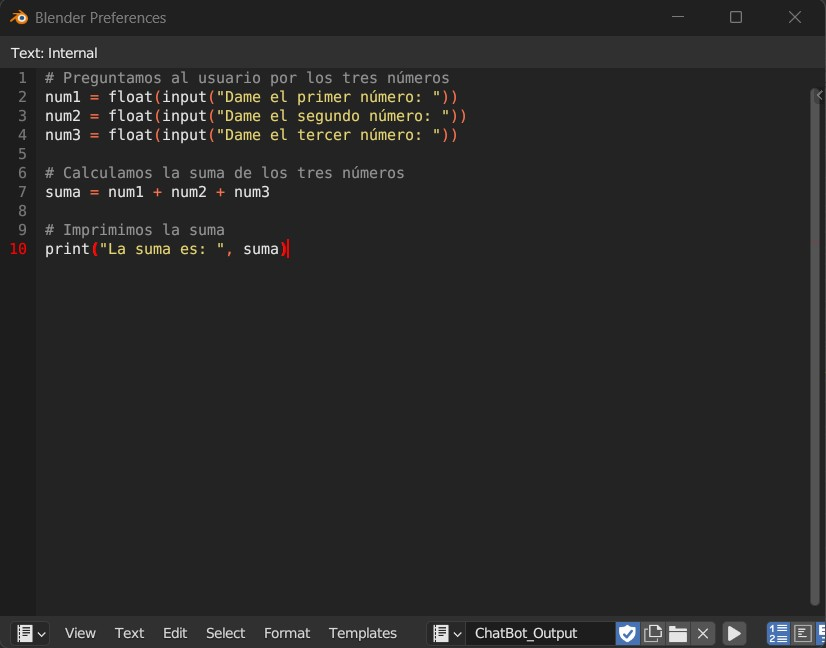
\includegraphics[width=0.8\textwidth]{figs/cu2_2.jpg}
    \caption{Captura de pantalla del código generado en el panel de scripting de Blender para el CU2 en las pruebas funcionales}
    \label{fig:cu2_2}
  \end{figure}

% Imagen
  \begin{figure}[h!tb]
    \centering
    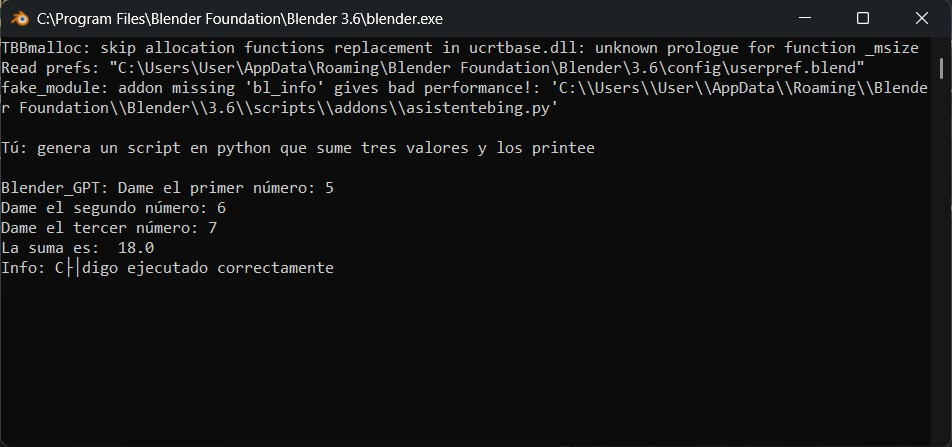
\includegraphics[width=0.8\textwidth]{figs/cu2_3.jpg}
    \caption{Captura de pantalla del código ejecutado en el terminal de Blender para el CU2 en las pruebas funcionales}
    \label{fig:cu2_3}
  \end{figure}

% Imagen
  \begin{figure}[h!tb]
    \centering
    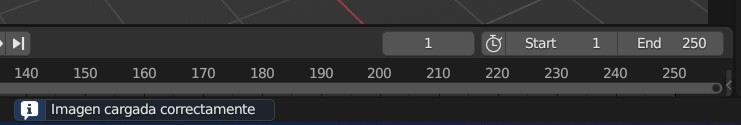
\includegraphics[width=0.8\textwidth]{figs/cu3.jpg}
    \caption{Captura de pantalla de la barra de notificaciones de blender para el CU3 en las pruebas funcionales}
    \label{fig:cu3}
  \end{figure}

% Imagen
  \begin{figure}[h!tb]
    \centering
    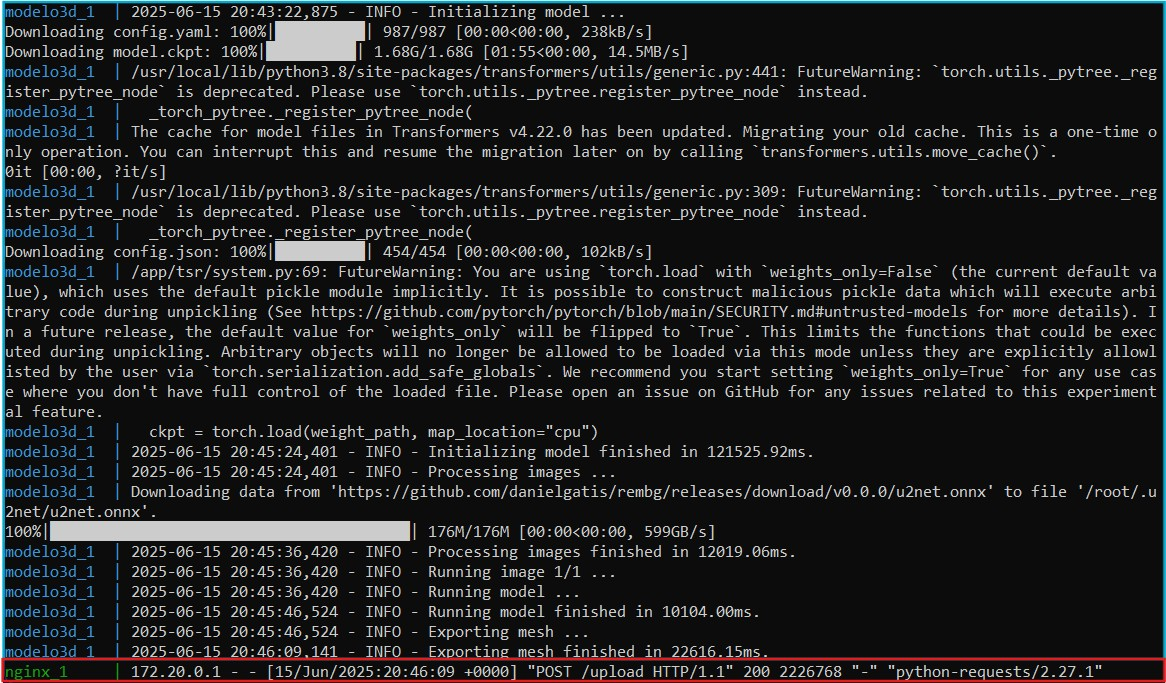
\includegraphics[width=0.8\textwidth]{figs/cu4cu9.jpg}
    \caption{Captura de pantalla del terminal de logs del servidor para el CU4 y CU9 en las pruebas funcionales}
    \label{fig:cu4cu9}
  \end{figure}

% Imagen
  \begin{figure}[h!tb]
    \centering
    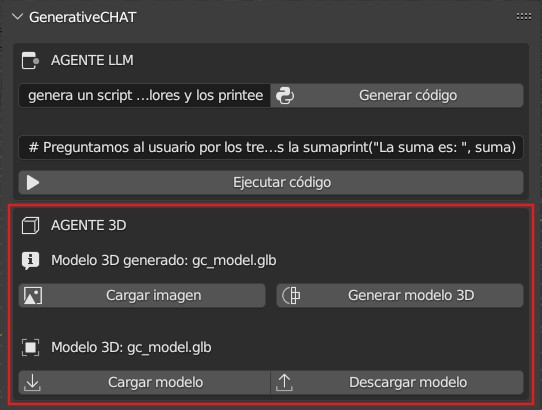
\includegraphics[width=0.8\textwidth]{figs/cu5_1.jpg}
    \caption{Captura de pantalla del add-on con el modelo 3D generado para el CU5 en las pruebas funcionales}
    \label{fig:cu5_1}
  \end{figure}

% Imagen
  \begin{figure}[h!tb]
    \centering
    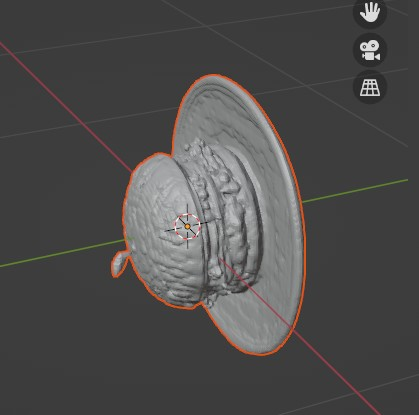
\includegraphics[width=0.8\textwidth]{figs/cu5_2.jpg}
    \caption{Captura de pantalla del modelo 3D cargado en la escena de Blender para el CU5 en las pruebas funcionales}
    \label{fig:cu5_2}
  \end{figure}

% Imagen
  \begin{figure}[h!tb]
    \centering
    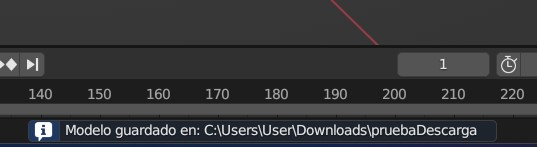
\includegraphics[width=0.8\textwidth]{figs/cu6_1.jpg}
    \caption{Captura de pantalla de la barra de notificaciones de blender para el CU6 en las pruebas funcionales}
    \label{fig:cu6_1}
  \end{figure}

% Imagen
  \begin{figure}[h!tb]
    \centering
    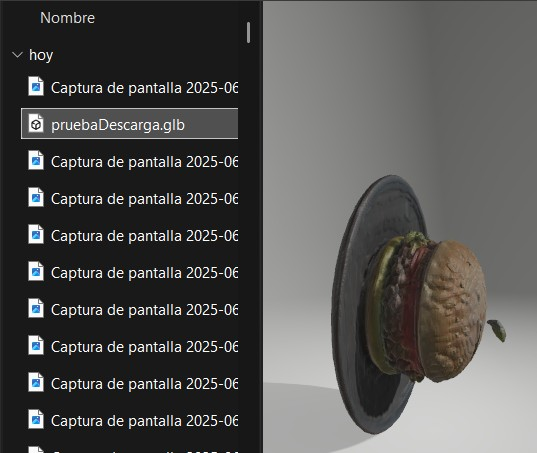
\includegraphics[width=0.8\textwidth]{figs/cu6_2.jpg}
    \caption{Captura de pantalla de la carpeta de descargas con el modelo 3D exportado para el CU6 en las pruebas funcionales}
    \label{fig:cu6_2}
  \end{figure}

% Imagen
  \begin{figure}[h!tb]
    \centering
    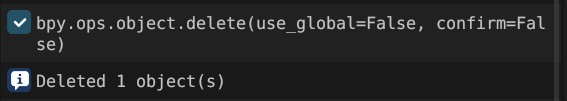
\includegraphics[width=0.8\textwidth]{figs/cu7.jpg}
    \caption{Captura de pantalla del terminal de blender despues de revertir la eliminación de un objeto para el CU7 en las pruebas funcionales}
    \label{fig:cu7}
  \end{figure}


\clearpage
\section{Resultados de las pruebas de rendimiento}
\label{sec:puntoC2}

% Imagen R1
  \begin{figure}[h!tb]
    \centering
    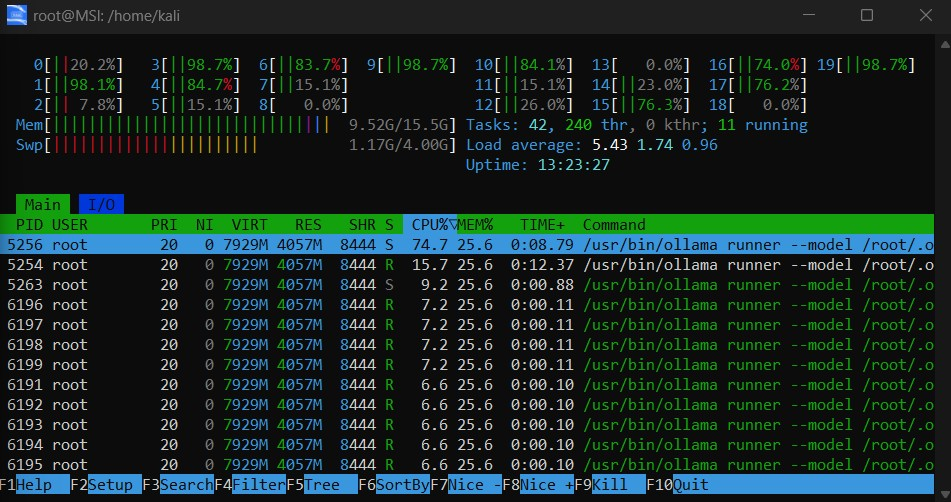
\includegraphics[width=0.8\textwidth]{figs/LLM1.jpg}
    \caption{Resultado de la prueba de rendimiento con 1 petición sobre el microservicio del modelo LLM}
    \label{fig:resRend1LLM}
  \end{figure}

% Imagen R5
  \begin{figure}[h!tb]
    \centering
    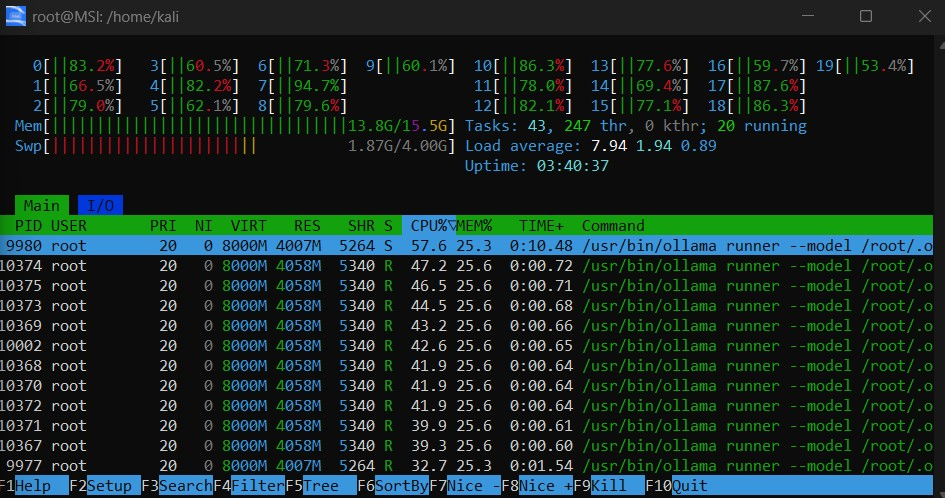
\includegraphics[width=0.8\textwidth]{figs/LLM2.jpg}
    \caption{Resultado de la prueba de rendimiento con 2 petición sobre el microservicio del modelo LLM}
    \label{fig:resRend2LLM}
  \end{figure}

% Imagen R6
  \begin{figure}[h!tb]
    \centering
    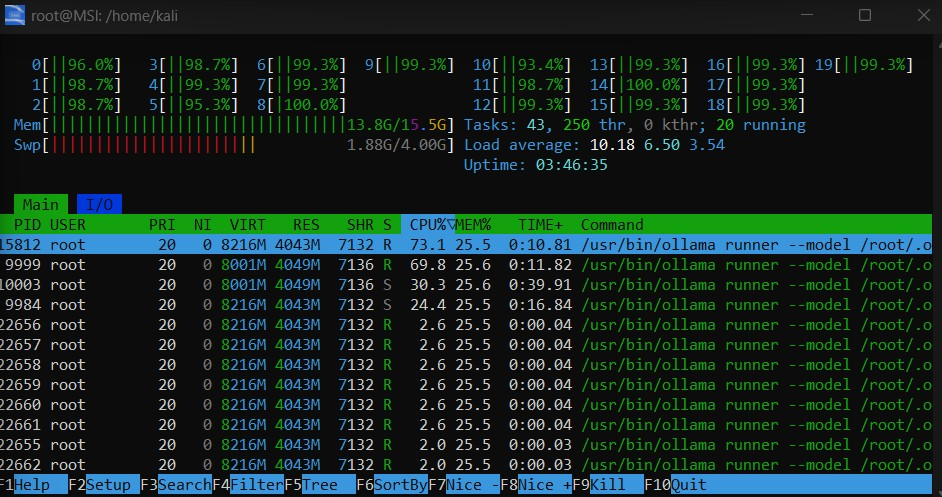
\includegraphics[width=0.8\textwidth]{figs/LLM3.jpg}
    \caption{Resultado de la prueba de rendimiento con 3 petición sobre el microservicio del modelo LLM}
    \label{fig:resRend3LLM}
  \end{figure}

% Imagen R2
  \begin{figure}[h!tb]
    \centering
    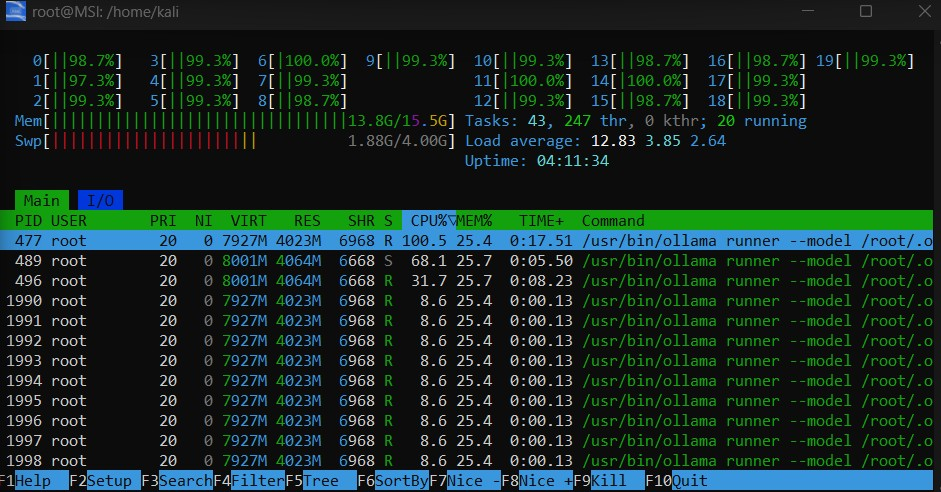
\includegraphics[width=0.8\textwidth]{figs/LLM4.jpg}
    \caption{Resultado de la prueba de rendimiento con 4 petición sobre el microservicio del modelo LLM}
    \label{fig:resRend4LLM}
  \end{figure}

% Imagen R3
  \begin{figure}[h!tb]
    \centering
    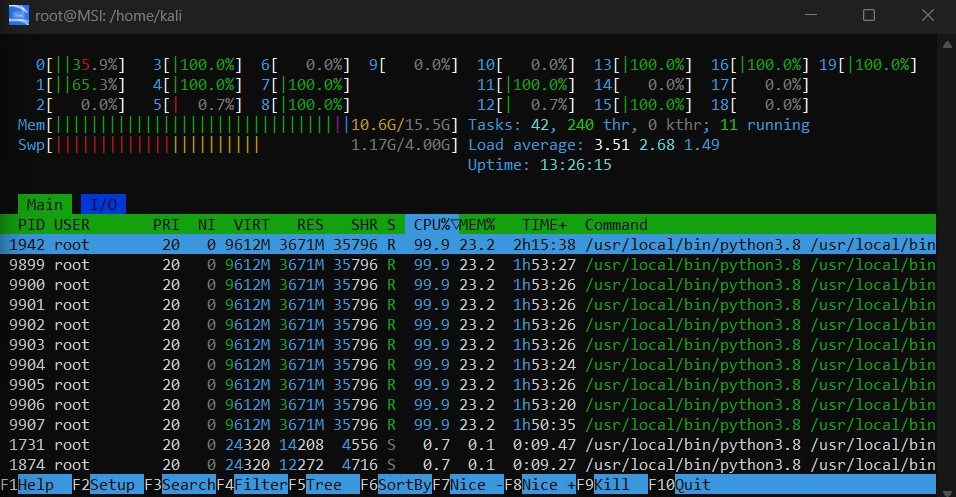
\includegraphics[width=0.8\textwidth]{figs/3D1.jpg}
    \caption{Resultado de la prueba de rendimiento con 1 petición sobre el microservicio del modelo 3D TripoSR}
    \label{fig:resRend13D}
  \end{figure}

% Imagen R7
  \begin{figure}[h!tb]
    \centering
    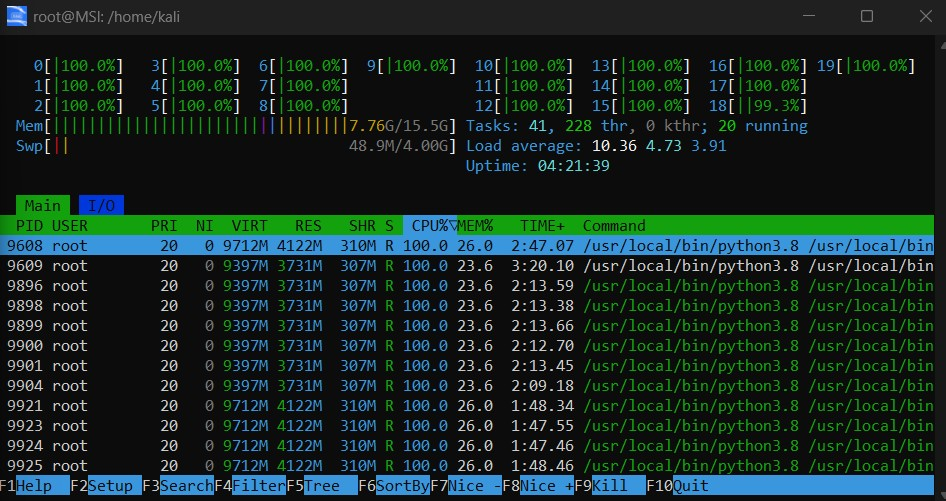
\includegraphics[width=0.8\textwidth]{figs/3D2.jpg}
    \caption{Resultado de la prueba de rendimiento con 2 petición sobre el microservicio del modelo 3D TripoSR}
    \label{fig:resRend23D}
  \end{figure}

% Imagen R8
  \begin{figure}[h!tb]
    \centering
    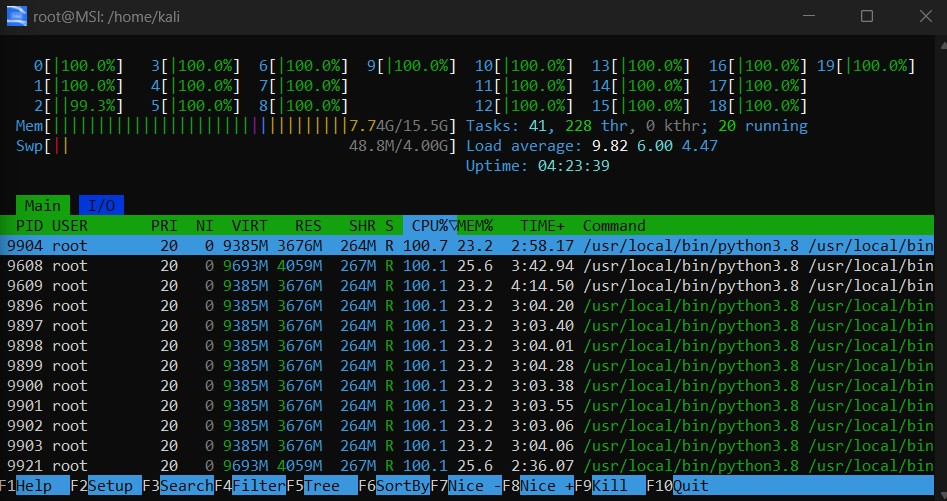
\includegraphics[width=0.8\textwidth]{figs/3D3.jpg}
    \caption{Resultado de la prueba de rendimiento con 3 petición sobre el microservicio del modelo 3D TripoSR}
    \label{fig:resRend33D}
  \end{figure}

% Imagen R4
  \begin{figure}[h!tb]
    \centering
    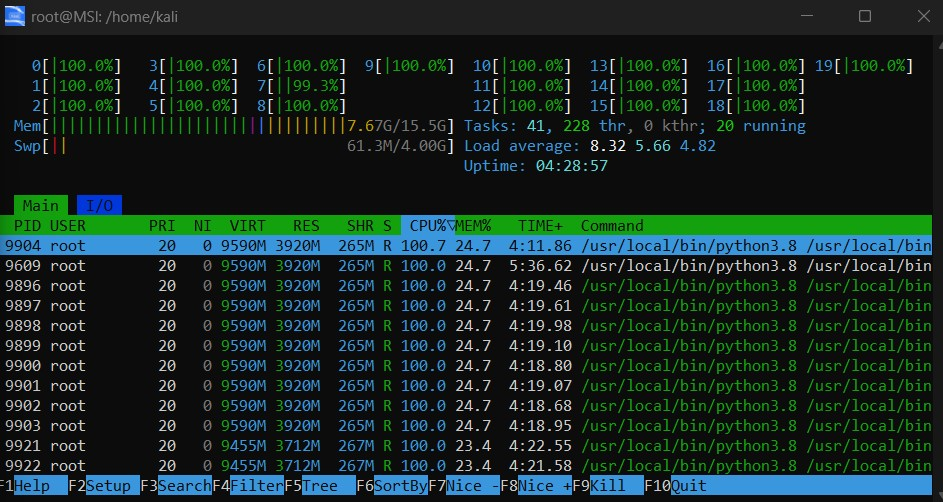
\includegraphics[width=0.8\textwidth]{figs/3D4.jpg}
    \caption{Resultado de la prueba de rendimiento con 4 petición sobre el microservicio del modelo 3D TripoSR}
    \label{fig:resRend43D}
  \end{figure}
